% Options for packages loaded elsewhere
\PassOptionsToPackage{unicode}{hyperref}
\PassOptionsToPackage{hyphens}{url}
\PassOptionsToPackage{dvipsnames,svgnames,x11names}{xcolor}
%
\documentclass[
  10pt,
  ignorenonframetext,
]{beamer}
\usepackage{pgfpages}
\setbeamertemplate{caption}[numbered]
\setbeamertemplate{caption label separator}{: }
\setbeamercolor{caption name}{fg=normal text.fg}
\beamertemplatenavigationsymbolsempty
% Prevent slide breaks in the middle of a paragraph
\widowpenalties 1 10000
\raggedbottom
\setbeamertemplate{part page}{
  \centering
  \begin{beamercolorbox}[sep=16pt,center]{part title}
    \usebeamerfont{part title}\insertpart\par
  \end{beamercolorbox}
}
\setbeamertemplate{section page}{
  \centering
  \begin{beamercolorbox}[sep=12pt,center]{part title}
    \usebeamerfont{section title}\insertsection\par
  \end{beamercolorbox}
}
\setbeamertemplate{subsection page}{
  \centering
  \begin{beamercolorbox}[sep=8pt,center]{part title}
    \usebeamerfont{subsection title}\insertsubsection\par
  \end{beamercolorbox}
}
\AtBeginPart{
  \frame{\partpage}
}
\AtBeginSection{
  \ifbibliography
  \else
    \frame{\sectionpage}
  \fi
}
\AtBeginSubsection{
  \frame{\subsectionpage}
}
\usepackage{amsmath,amssymb}
\usepackage{iftex}
\ifPDFTeX
  \usepackage[T1]{fontenc}
  \usepackage[utf8]{inputenc}
  \usepackage{textcomp} % provide euro and other symbols
\else % if luatex or xetex
  \usepackage{unicode-math} % this also loads fontspec
  \defaultfontfeatures{Scale=MatchLowercase}
  \defaultfontfeatures[\rmfamily]{Ligatures=TeX,Scale=1}
\fi
\usepackage{lmodern}
\usetheme[]{Singapore}
\usefonttheme{serif}
\ifPDFTeX\else
  % xetex/luatex font selection
\fi
% Use upquote if available, for straight quotes in verbatim environments
\IfFileExists{upquote.sty}{\usepackage{upquote}}{}
\IfFileExists{microtype.sty}{% use microtype if available
  \usepackage[]{microtype}
  \UseMicrotypeSet[protrusion]{basicmath} % disable protrusion for tt fonts
}{}
\makeatletter
\@ifundefined{KOMAClassName}{% if non-KOMA class
  \IfFileExists{parskip.sty}{%
    \usepackage{parskip}
  }{% else
    \setlength{\parindent}{0pt}
    \setlength{\parskip}{6pt plus 2pt minus 1pt}}
}{% if KOMA class
  \KOMAoptions{parskip=half}}
\makeatother
\usepackage{xcolor}
\newif\ifbibliography
\usepackage{color}
\usepackage{fancyvrb}
\newcommand{\VerbBar}{|}
\newcommand{\VERB}{\Verb[commandchars=\\\{\}]}
\DefineVerbatimEnvironment{Highlighting}{Verbatim}{commandchars=\\\{\}}
% Add ',fontsize=\small' for more characters per line
\usepackage{framed}
\definecolor{shadecolor}{RGB}{248,248,248}
\newenvironment{Shaded}{\begin{snugshade}}{\end{snugshade}}
\newcommand{\AlertTok}[1]{\textcolor[rgb]{0.94,0.16,0.16}{#1}}
\newcommand{\AnnotationTok}[1]{\textcolor[rgb]{0.56,0.35,0.01}{\textbf{\textit{#1}}}}
\newcommand{\AttributeTok}[1]{\textcolor[rgb]{0.13,0.29,0.53}{#1}}
\newcommand{\BaseNTok}[1]{\textcolor[rgb]{0.00,0.00,0.81}{#1}}
\newcommand{\BuiltInTok}[1]{#1}
\newcommand{\CharTok}[1]{\textcolor[rgb]{0.31,0.60,0.02}{#1}}
\newcommand{\CommentTok}[1]{\textcolor[rgb]{0.56,0.35,0.01}{\textit{#1}}}
\newcommand{\CommentVarTok}[1]{\textcolor[rgb]{0.56,0.35,0.01}{\textbf{\textit{#1}}}}
\newcommand{\ConstantTok}[1]{\textcolor[rgb]{0.56,0.35,0.01}{#1}}
\newcommand{\ControlFlowTok}[1]{\textcolor[rgb]{0.13,0.29,0.53}{\textbf{#1}}}
\newcommand{\DataTypeTok}[1]{\textcolor[rgb]{0.13,0.29,0.53}{#1}}
\newcommand{\DecValTok}[1]{\textcolor[rgb]{0.00,0.00,0.81}{#1}}
\newcommand{\DocumentationTok}[1]{\textcolor[rgb]{0.56,0.35,0.01}{\textbf{\textit{#1}}}}
\newcommand{\ErrorTok}[1]{\textcolor[rgb]{0.64,0.00,0.00}{\textbf{#1}}}
\newcommand{\ExtensionTok}[1]{#1}
\newcommand{\FloatTok}[1]{\textcolor[rgb]{0.00,0.00,0.81}{#1}}
\newcommand{\FunctionTok}[1]{\textcolor[rgb]{0.13,0.29,0.53}{\textbf{#1}}}
\newcommand{\ImportTok}[1]{#1}
\newcommand{\InformationTok}[1]{\textcolor[rgb]{0.56,0.35,0.01}{\textbf{\textit{#1}}}}
\newcommand{\KeywordTok}[1]{\textcolor[rgb]{0.13,0.29,0.53}{\textbf{#1}}}
\newcommand{\NormalTok}[1]{#1}
\newcommand{\OperatorTok}[1]{\textcolor[rgb]{0.81,0.36,0.00}{\textbf{#1}}}
\newcommand{\OtherTok}[1]{\textcolor[rgb]{0.56,0.35,0.01}{#1}}
\newcommand{\PreprocessorTok}[1]{\textcolor[rgb]{0.56,0.35,0.01}{\textit{#1}}}
\newcommand{\RegionMarkerTok}[1]{#1}
\newcommand{\SpecialCharTok}[1]{\textcolor[rgb]{0.81,0.36,0.00}{\textbf{#1}}}
\newcommand{\SpecialStringTok}[1]{\textcolor[rgb]{0.31,0.60,0.02}{#1}}
\newcommand{\StringTok}[1]{\textcolor[rgb]{0.31,0.60,0.02}{#1}}
\newcommand{\VariableTok}[1]{\textcolor[rgb]{0.00,0.00,0.00}{#1}}
\newcommand{\VerbatimStringTok}[1]{\textcolor[rgb]{0.31,0.60,0.02}{#1}}
\newcommand{\WarningTok}[1]{\textcolor[rgb]{0.56,0.35,0.01}{\textbf{\textit{#1}}}}
\usepackage{longtable,booktabs,array}
\usepackage{calc} % for calculating minipage widths
\usepackage{caption}
% Make caption package work with longtable
\makeatletter
\def\fnum@table{\tablename~\thetable}
\makeatother
\usepackage{graphicx}
\makeatletter
\def\maxwidth{\ifdim\Gin@nat@width>\linewidth\linewidth\else\Gin@nat@width\fi}
\def\maxheight{\ifdim\Gin@nat@height>\textheight\textheight\else\Gin@nat@height\fi}
\makeatother
% Scale images if necessary, so that they will not overflow the page
% margins by default, and it is still possible to overwrite the defaults
% using explicit options in \includegraphics[width, height, ...]{}
\setkeys{Gin}{width=\maxwidth,height=\maxheight,keepaspectratio}
% Set default figure placement to htbp
\makeatletter
\def\fps@figure{htbp}
\makeatother
\setlength{\emergencystretch}{3em} % prevent overfull lines
\providecommand{\tightlist}{%
  \setlength{\itemsep}{0pt}\setlength{\parskip}{0pt}}
\setcounter{secnumdepth}{-\maxdimen} % remove section numbering
\newlength{\cslhangindent}
\setlength{\cslhangindent}{1.5em}
\newlength{\csllabelwidth}
\setlength{\csllabelwidth}{3em}
\newlength{\cslentryspacingunit} % times entry-spacing
\setlength{\cslentryspacingunit}{\parskip}
\newenvironment{CSLReferences}[2] % #1 hanging-ident, #2 entry spacing
 {% don't indent paragraphs
  \setlength{\parindent}{0pt}
  % turn on hanging indent if param 1 is 1
  \ifodd #1
  \let\oldpar\par
  \def\par{\hangindent=\cslhangindent\oldpar}
  \fi
  % set entry spacing
  \setlength{\parskip}{#2\cslentryspacingunit}
 }%
 {}
\usepackage{calc}
\newcommand{\CSLBlock}[1]{#1\hfill\break}
\newcommand{\CSLLeftMargin}[1]{\parbox[t]{\csllabelwidth}{#1}}
\newcommand{\CSLRightInline}[1]{\parbox[t]{\linewidth - \csllabelwidth}{#1}\break}
\newcommand{\CSLIndent}[1]{\hspace{\cslhangindent}#1}
\usepackage{multirow}
\ifLuaTeX
  \usepackage{selnolig}  % disable illegal ligatures
\fi
\IfFileExists{bookmark.sty}{\usepackage{bookmark}}{\usepackage{hyperref}}
\IfFileExists{xurl.sty}{\usepackage{xurl}}{} % add URL line breaks if available
\urlstyle{same}
\hypersetup{
  pdftitle={Module 5: Resampling},
  pdfauthor={Sara Martino, Department of Mathematical Sciences, NTNU},
  colorlinks=true,
  linkcolor={Maroon},
  filecolor={Maroon},
  citecolor={Blue},
  urlcolor={blue},
  pdfcreator={LaTeX via pandoc}}

\title{Module 5: Resampling}
\subtitle{TMA4268 Statistical Learning V2023}
\author{Sara Martino, Department of Mathematical Sciences, NTNU}
\date{February 8 and 9, 2023}

\begin{document}
\frame{\titlepage}

\begin{frame}{Acknowledgements}
\protect\hypertarget{acknowledgements}{}
\begin{itemize}
\item
  A lot of this material stems from Mette Langaas and her TAs. I would
  like to thank Mette for the permission to use her material!
\item
  Some of the figures and slides in this presentation are taken (or are
  inspired) from James et al. (2013).
\end{itemize}
\end{frame}

\begin{frame}{Introduction}
\protect\hypertarget{introduction}{}
\begin{block}{Learning material for this module}
\protect\hypertarget{learning-material-for-this-module}{}
\vspace{2mm}

\begin{itemize}
\item
  James et al (2021): An Introduction to Statistical Learning, Chapter
  5.
\item
  All the material presented on these module slides.
\end{itemize}

\vspace{2mm}

Additional material for the interested reader: Chapter 7 (in particular
7.10) in Friedman et al (2001): Elements of Statistical learning.
\end{block}
\end{frame}

\begin{frame}
\begin{block}{What will you learn?}
\protect\hypertarget{what-will-you-learn}{}
\(~\)

\begin{itemize}
\tightlist
\item
  What is model assessment and model selection?
\end{itemize}

\vspace{2mm}

\begin{itemize}
\tightlist
\item
  Ideal solution in a data rich situation.
\end{itemize}

\vspace{2mm}

\begin{itemize}
\tightlist
\item
  Cross-validation and what is best:

  \begin{itemize}
  \tightlist
  \item
    validation set
  \item
    leave-one-out cross-validation (LOOCV)
  \item
    \(k\)-fold CV
  \end{itemize}
\end{itemize}

\vspace{2mm}

\begin{itemize}
\tightlist
\item
  Bootstrapping - how and why.
\end{itemize}
\end{block}
\end{frame}

\begin{frame}{Performance of a learning method}
\protect\hypertarget{performance-of-a-learning-method}{}
\begin{itemize}
\item
  Our models are ``good'' when they can generalize.
\item
  We want a learning method to perform well on new data (low test
  error).
\item
  Inference and understanding of the true pattern (in contrast to
  overfitting)
\end{itemize}

\vspace{2mm}

This is important both for

\textbf{Model selection}

Estimate the \emph{performance} of different models to \emph{choose the
best model}.

\textbf{Model assessment}

Estimating the performance (prediction error) of the final model, on new
data.
\end{frame}

\begin{frame}
\begin{block}{Training vs Test Error}
\protect\hypertarget{training-vs-test-error}{}
\(~\)

\centering

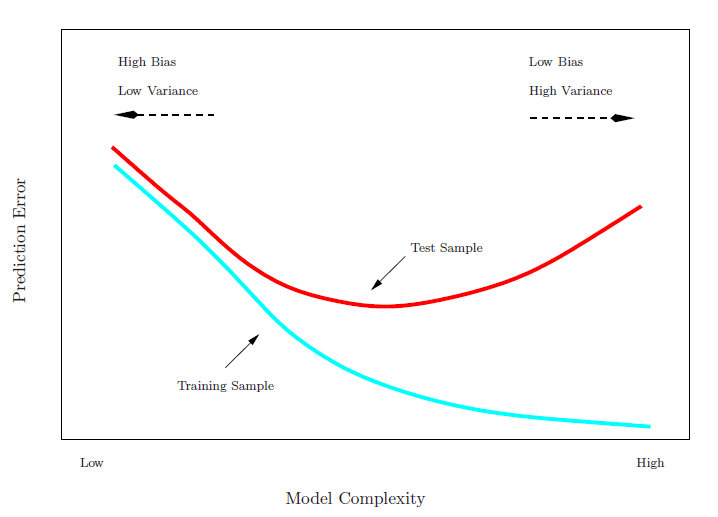
\includegraphics[width=0.8\textwidth,height=\textheight]{training_test.png}
\end{block}
\end{frame}

\begin{frame}
\begin{block}{Loss functions}
\protect\hypertarget{loss-functions}{}
\(~\)

In order to define how we measure error, we must first decide for a
\textbf{loss function}. Here we use:

\vspace{2mm}

\begin{itemize}
\tightlist
\item
  \emph{\textcolor{red}{Mean squared error}} (quadratic loss) for
  regression problems (continuous outcomes)
  \(Y_i=f({\boldsymbol x}_i)+\varepsilon_i\), \(i=1,\ldots, n\):
\end{itemize}

\[\text{MSE}=\frac{1}{n}\sum_{i=1}^n (y_i-\hat{f}({\boldsymbol x}_i))^2 \ .\]

\vspace{2mm}

\begin{itemize}
\tightlist
\item
  \emph{\textcolor{red}{Misclassification rate}} (0/1 loss) for
  classification problems where we classify to the class with the
  highest probability \(P(Y=j\mid {\boldsymbol x}_0)\) for
  \(j=1,\ldots,K\):
  \[\frac{1}{n}\sum_{i=1}^n \text{I}(y_i \neq \hat{y}_i) \ .\]
\end{itemize}

\vspace{2mm}

\textbf{NB:} These are just two of the possible loss functions, there
are several model to be found in the literature
\end{block}
\end{frame}

\begin{frame}
\begin{block}{KNN regression (chapter 3.5 in course book)}
\protect\hypertarget{knn-regression-chapter-3.5-in-course-book}{}
\vspace{2mm}

\begin{itemize}
\tightlist
\item
  The KNN regression method provides a prediction at a value \(x_0\) by
  finding the closest \(K\) points (Euclidean distance) and calculating
  the average of the observed \(y\) values at the points in the
  respective neighborhood \(\mathcal{N}_0\)
\end{itemize}

\[\hat{f}(x_0)=\frac{1}{K}\sum_{i\in \mathcal{N}_0} y_i \ .\]

\(~\)

Illustration: Linear regression with \(K=1\) (left) and \(K=9\) (right).

\centering

\includegraphics[width=0.55\textwidth,height=\textheight]{../../ISLR/Figures/Chapter3/3.17.pdf}

\tiny

(Figure 3.17 from James et al. (2013)).

\(~\)

\normalsize
\flushleft

What happens for \(K=\) number of data points?
\end{block}
\end{frame}

\begin{frame}
\begin{block}{Example}
\protect\hypertarget{example}{}
\vspace{2mm}

We aim to do \emph{model selection} in KNN-regression, where true curve
is \(f(x)=-x+x^2+x^3\) with \(x \in [-3,3]\). \(n=61\) for the training
data.

\vspace{4mm}

\centering

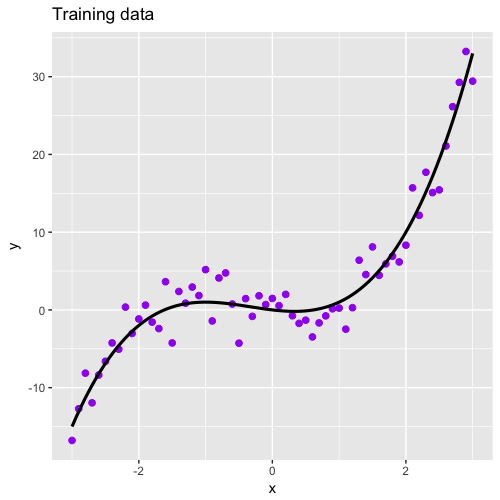
\includegraphics[width=0.5\textwidth,height=\textheight]{Prob1f1.png}

\begin{itemize}
\tightlist
\item
  We have considered \(K=1,\ldots,25\), and repeated the experiment
  \(M=1000\) times (that is, \(M\) versions of training and test set).
\end{itemize}
\end{block}
\end{frame}

\begin{frame}
\begin{block}{Remember: The bias-variance trade-off}
\protect\hypertarget{remember-the-bias-variance-trade-off}{}
\vspace{2mm}

For KNN: \(K\) small = high complexity; \(K\) large = low complexity.

\vspace{2mm}

\centering

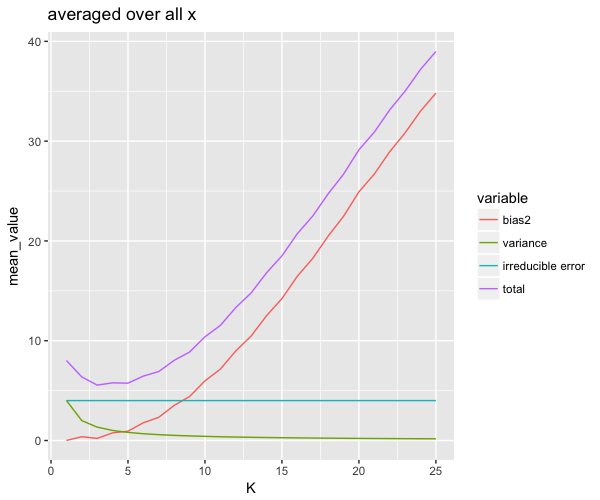
\includegraphics[width=0.75\textwidth,height=\textheight]{Prob1f4.png}
\end{block}
\end{frame}

\begin{frame}
\begin{block}{The challenge}
\protect\hypertarget{the-challenge}{}
\(~\)

\begin{itemize}
\tightlist
\item
  In the above examples we knew the truth, so we could assess training
  and test error.
\end{itemize}

\vspace{2mm}

\begin{itemize}
\tightlist
\item
  In reality this is of course not the case.
\end{itemize}

\vspace{2mm}

\begin{itemize}
\tightlist
\item
  We need approaches that work with real data!
\end{itemize}
\end{block}
\end{frame}

\begin{frame}
\begin{block}{The data-rich situation (often unrealistic)}
\protect\hypertarget{the-data-rich-situation-often-unrealistic}{}
\vspace{2mm}

If we had a large amount of data we could divide our data into three
parts:

\begin{itemize}
\tightlist
\item
  \textbf{Training set}: to fit the model
\item
  \textbf{Validation set}: to select the best model (\emph{model
  selection})
\item
  \textbf{Test set}: to assess how well the model fits on new
  independent data (\emph{model assessment})
\end{itemize}

\vspace{2mm}

\textbf{Q}: Before we had just training and test. Why do we need the
additional validation set?

\textbf{A}: We have not discussed model selection before.

\vspace{2mm}

\textbf{Q}: Why can't we just use the training set for training, and
then the test set both for model selection and for model evaluation?

\textbf{A}: We will be too optimistic if we report the error on the test
set when we have already used the test set to choose the best model.
\end{block}
\end{frame}

\begin{frame}
\begin{itemize}
\item
  If you have a lot of data -- great -- then you do not need Module 5.
\item
  But, this is very seldom the case -- so we will study other solutions
  based on efficient sample reuse with \emph{resampling} data.
\item
  An alternative strategy for model selection (using methods penalizing
  model complexity, e.g.~AIC or lasso) is covered in Module 6.
\end{itemize}

We will look at \emph{cross-validation} and the \emph{bootstrap}.
\end{frame}

\begin{frame}{Cross-validation (CV)}
\protect\hypertarget{cross-validation-cv}{}
\(~\)

``Model selection'' situation: We assume that test data is available
(and has been put aside), and we want to use the rest of our data to
find the model that performs ``best'', that is, \emph{with lowest test
error}.

\vspace{2mm}

This can be done by:

\begin{itemize}
\tightlist
\item
  the validation set approach (not strictly a \emph{cross}-validation
  approach).
\item
  leave one out cross-validation (LOOCV).
\item
  \(k\)-fold cross-validation (CV), typically \(k=5\) or \(10\).
\end{itemize}
\end{frame}

\begin{frame}
\begin{block}{The validation set approach}
\protect\hypertarget{the-validation-set-approach}{}
\vspace{2mm}

\begin{itemize}
\item
  Consider the case when you have a data set consisting of \(n\)
  observations.
\item
  To fit a model and to evaluate its predictive performance you randomly
  divide the data set into two parts (\(n/2\) sample size each):

  \begin{itemize}
  \tightlist
  \item
    a \emph{training set} (to fit the model) and
  \item
    a \emph{validation set} (to make predictions of the response
    variable for the observations in the validation set)
  \end{itemize}
\end{itemize}

\vspace{4mm}

\includegraphics{../../ISLR/Figures/Chapter5/5.1.pdf}
\end{block}
\end{frame}

\begin{frame}[fragile]
\begin{block}{Example of validation set approach}
\protect\hypertarget{example-of-validation-set-approach}{}
\vspace{2mm}

Auto data set (library \texttt{ISLR}): predict \texttt{mpg} (miles pr
gallon) using polynomial function of \texttt{horsepower} (of engine),
\(n=392\). What do you see?

\begin{center}\includegraphics[width=0.7\linewidth]{5Resample_files/figure-beamer/chunkName-1} \end{center}
\end{block}
\end{frame}

\begin{frame}
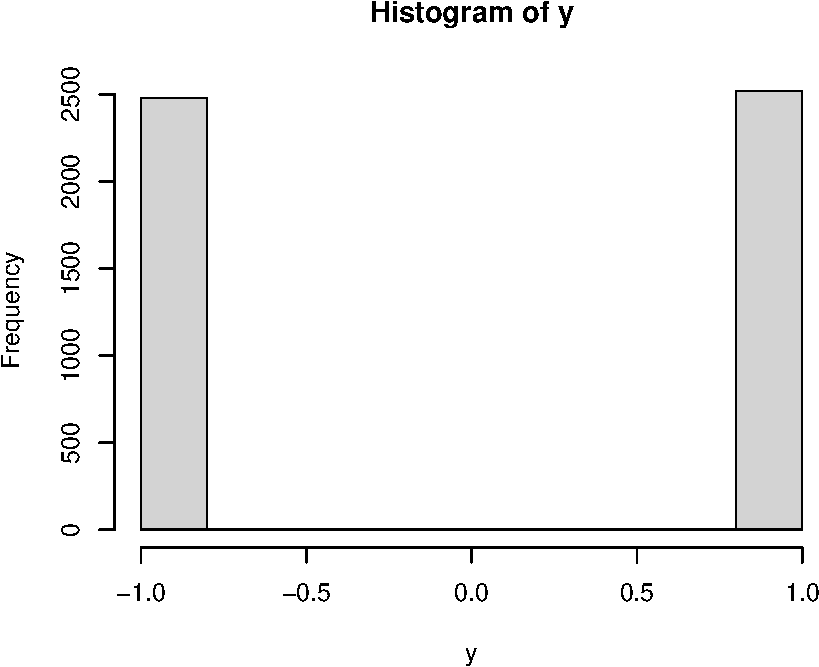
\includegraphics[width=0.7\linewidth]{5Resample_files/figure-beamer/unnamed-chunk-1-1}
\end{frame}

\begin{frame}
But what if we select another split into two parts? Many splits:

\begin{center}\includegraphics[width=0.7\linewidth]{5Resample_files/figure-beamer/auto2-1} \end{center}

\vspace{2mm}

\(\rightarrow\) No consensus which model really gives the lowest
validation set MSE.
\end{frame}

\begin{frame}
\begin{block}{Drawbacks with the validation set approach}
\protect\hypertarget{drawbacks-with-the-validation-set-approach}{}
\vspace{2mm}

\begin{itemize}
\tightlist
\item
  \emph{\textcolor{red}{High variability}} of validation set error due
  to dependency on the set of observation included in the training and
  validation set.
\end{itemize}

\vspace{2mm}

\begin{itemize}
\tightlist
\item
  \emph{\textcolor{red}{Smaller sample size}} for model fit, as only
  half of the observations are in the training set. Therefore, the
  validation set error may tend to overestimate the error rate on new
  observations for a model that is fit on the full data set (the more
  data, the lower the error).
\end{itemize}
\end{block}
\end{frame}

\begin{frame}
Better ideas?
\end{frame}

\begin{frame}
\begin{block}{Leave-one-out cross-validation (LOOCV)}
\protect\hypertarget{leave-one-out-cross-validation-loocv}{}
\(~\)

Leave-one-out cross-validation (LOOCV) addresses the limitations of the
validation set approach.

\vspace{4mm}

\textbf{Idea:}

\begin{itemize}
\tightlist
\item
  Only \textbf{one observation at a time} is left out (test set size
  \(n=1\)).
\item
  The remaining \(n-1\) observations make up the training set.
\item
  The procedure of model fitting is repeated \(n\) times, such that each
  of the \(n\) observations is left out once. In each step, we calculate
\end{itemize}

\[\text{MSE}_i=(y_i-\hat{y}_i)^2 \ .\]

\begin{itemize}
\tightlist
\item
  The \textbf{total prediction error} is the mean across these \(n\)
  models
\end{itemize}

\[\text{CV}_{n}=\frac{1}{n}\sum_{i=1}^n \text{MSE}_i \ .\]
\end{block}
\end{frame}

\begin{frame}
\begin{block}{Regression example: LOOCV}
\protect\hypertarget{regression-example-loocv}{}
\begin{center}\includegraphics[width=0.7\linewidth]{5Resample_files/figure-beamer/auto_loocv-1} \end{center}

\tiny

\normalsize
\end{block}
\end{frame}

\begin{frame}
\begin{block}{Issues with leave-one-out cross-validation}
\protect\hypertarget{issues-with-leave-one-out-cross-validation}{}
\(~\)

\begin{itemize}
\tightlist
\item
  Pros:

  \begin{itemize}
  \tightlist
  \item
    No randomness in training/validation splits!
  \item
    Little bias, since nearly the whole data set used for training
    (compared to half for validation set approach).
  \end{itemize}
\end{itemize}

\vspace{2mm}

\begin{itemize}
\tightlist
\item
  Cons:

  \begin{itemize}
  \tightlist
  \item
    Expensive to implement -- need to fit \(n\) different models.
  \item
    High variance since: two training sets only differ by one
    observation, thus estimates from each fold highly correlated, which
    can lead to high variance in their average\(^\star\).
  \end{itemize}
\end{itemize}

\vspace{5mm}
\scriptsize

\(^\star\) Recall that
\[\text{Var}(\sum_{i=1}^na_iX_i)=\sum_{i=1}^n\sum_{j=1}^n a_ia_j\text{Cov}(X_i,X_j)\]
\[=\sum_{i=1}^na_i^2\text{Var}(X_i)+2\sum_{i=2}^n \sum_{j=1}^{i-1}
a_ia_j\text{Cov}(X_i,X_j).\]
\end{block}
\end{frame}

\begin{frame}
\begin{block}{LOOCV for multiple linear regression}
\protect\hypertarget{loocv-for-multiple-linear-regression}{}
\vspace{2mm}

There is a nice shortcut for LOOCV in the case of linear regression:

\[ \text{CV}_{n}=\frac{1}{n}\sum_{i=1}^n \left( \frac{y_i-\hat{y}_i}{1-h_{ii}} \right) ^2 \ ,\]

where \(h_i\) is the \(i\)th diagonal element (leverage) of the hat
matrix \({\bf H}={\bf X}({\bf X}^T{\bf X})^{-1}{\bf X}^T\), and
\(\hat{y}_i\) is the \(i\)th fitted value from the original least
squares fit.

\vspace{2mm}

\(\rightarrow\) Need to fit the model only once!

\(~\)

\(~\)
\end{block}
\end{frame}

\begin{frame}
\begin{block}{\(k\)-fold cross-validation}
\protect\hypertarget{k-fold-cross-validation}{}
\(~\)

To address the drawbacks of LOOCV, we can leave out not just one single
observation in each iteration, but \(1/k\)-th of all data.

\(~\)

\textbf{Procedure:}

\begin{itemize}
\tightlist
\item
  Split the data into \(k\) (more or less) equal parts.
\end{itemize}

\vspace{2mm}

\begin{itemize}
\tightlist
\item
  Use \(k-1\) parts to fit and the \(k\)th part to validate.
\end{itemize}

\vspace{2mm}

\begin{itemize}
\tightlist
\item
  Do this \(k\) times and leave out another part in each round.
\end{itemize}

\(~\)

The MSE is then estimated in each of the \(k\) iterations
(\(\text{MSE}_1,\ldots,\text{MSE}_k\)). The \(k\)-fold CV is then a
(weighted) avearge over the \(k\) MSEs.
\end{block}
\end{frame}

\begin{frame}
\textbf{Comparison of LOOCV and \(k\)-fold CV}:

\centering

LOOCV:

\includegraphics[width=0.7\textwidth,height=\textheight]{../../ISLR/Figures/Chapter5/5.3.pdf}

\(k\)-fold:

\includegraphics[width=0.7\textwidth,height=\textheight]{../../ISLR/Figures/Chapter5/5.5.pdf}
\end{frame}

\begin{frame}
\begin{block}{Formally}
\protect\hypertarget{formally}{}
\begin{itemize}
\tightlist
\item
  Indices of observations - divided into \(k\) folds:
  \(C_1, C_2, \ldots, C_k\).
\item
  \(n_j\) elements in fold \(j\). If \(n\) is a multiple of \(k\) then
  \(n_j=n/k\) for all folds.
\end{itemize}

\[\text{MSE}_j=\frac{1}{n_j}\sum_{i\in C_j}(y_i-\hat{y}_i)^2\] where
\(\hat{y}_i\) is the fit for observation \(i\) obtained from the data
with part \(j\) removed.

\[\text{CV}_{k}=\frac{1}{n} \sum_{j=1}^k n_j \text{MSE}_j\]

Observe: setting \(k=n\) gives LOOCV.
\end{block}
\end{frame}

\begin{frame}
\begin{block}{Regression example: \(5\) and \(10\)-fold
cross-validation}
\protect\hypertarget{regression-example-5-and-10-fold-cross-validation}{}
\(~\)

\begin{center}\includegraphics[width=0.7\linewidth]{5Resample_files/figure-beamer/auto_510fold-1} \end{center}

\normalsize
\end{block}
\end{frame}

\begin{frame}
10 reruns (different splits) of the 10-CV method - to see variability:

\begin{center}\includegraphics[width=0.7\linewidth]{5Resample_files/figure-beamer/auto_510fold_10-1} \end{center}

There still \emph{is} variability, but \emph{much less} than for
validation set approach.
\end{frame}

\begin{frame}
\begin{block}{Issues with \(k\)-fold cross-validation}
\protect\hypertarget{issues-with-k-fold-cross-validation}{}
\(~\)

\begin{enumerate}
\tightlist
\item
  The \emph{result may vary} according to how the folds are made, but
  the variation is in general lower than for the validation set
  approach.
\end{enumerate}

\vspace{2mm}

\begin{enumerate}
\setcounter{enumi}{1}
\tightlist
\item
  Computational load lower with \(k=5\) or \(10\) than LOOCV.
\end{enumerate}

\vspace{2mm}

\begin{enumerate}
\setcounter{enumi}{2}
\tightlist
\item
  The training set is \((k-1)/k\) times the size of the original data
  set - the estimate of the prediction error is biased upwards.
\end{enumerate}

\vspace{2mm}

\begin{enumerate}
\setcounter{enumi}{3}
\tightlist
\item
  This bias is the smallest when \(k=n\) (LOOCV), but we know that LOOCV
  has high variance.
\end{enumerate}

\vspace{2mm}

\begin{enumerate}
\setcounter{enumi}{4}
\tightlist
\item
  Due to the \emph{bias-variance-trade-off}, \(k\)-fold CV often gives
  more accurate estimates of the test error rate than does LOOCV.\\
  \(\rightarrow\) \(k=5\) or \(k=10\) is used as a compromise.
\end{enumerate}
\end{block}
\end{frame}

\begin{frame}
\begin{block}{Choosing the best model}
\protect\hypertarget{choosing-the-best-model}{}
\(~\)

\begin{itemize}
\tightlist
\item
  There is a model parameter (maybe \(K\) in KNN or the degree of the
  polynomial), say \(\theta\), involved to calculate \(\text{CV}_j\),
  \(j=1,\ldots, k\)
\end{itemize}

\vspace{2mm}

\begin{itemize}
\tightlist
\item
  Based on the CV vs \(\theta\)-plot we can choose the model with
  \emph{the smallest \({\text{CV}_k}\)} as our best model.
\end{itemize}

\vspace{2mm}

\begin{itemize}
\tightlist
\item
  We then fit this model using the whole data set (not the test part,
  that is still kept away), and evaluate the performance on the test
  set.
\end{itemize}
\end{block}
\end{frame}

\begin{frame}
\textbf{One standard error rule:}

Denote by \(\text{MSE}_j(\theta)\), \(j=1,\ldots, k\) the \(k\) parts of
the MSE that together give the \(\text{CV}_k\).

We can compute the sample standard deviation (standard error) of all
\(\text{MSE}_j(\theta)\), \(j=1,\ldots, k\)
\[\hat{\text{SE}}(\text{CV}_k(\theta))= \sqrt{\sum_{j=1}^k (\text{MSE}_j(\theta) - \overline{\text{MSE}}(\theta))/(k-1)} \, \]

for each value of the complexity parameter
\(\theta\).\footnote{Strictly speaking, this estimate is not quite valid. Why?}

The \emph{one standard error rule} is to choose the simplest model
(\emph{e.g.}, with lowest polynomial degree) within one standard error
of the minimal error.
\end{frame}

\begin{frame}
\begin{block}{\(k\)-fold cross-validation in classification}
\protect\hypertarget{k-fold-cross-validation-in-classification}{}
\vspace{3mm}

What do we need to change from our regression set-up?

\vspace{3mm}

\begin{itemize}
\tightlist
\item
  For LOOCV \(\hat{y}_i\) is the fit for observation \(i\) obtained from
  the data with observations \(i\) removed, and
  \({\text{Err}_i}=I(y_i\neq \hat{y}_i)\) . LOOCV is then
  \[\text{CV}_{n}=\frac{1}{n} \sum_{i=1}^n {\text{Err}_i}\]
\end{itemize}

\vspace{2mm}

\begin{itemize}
\tightlist
\item
  The \(k\)-fold CV is defined analogously.
\end{itemize}

\vspace{3mm}

\begin{itemize}
\tightlist
\item
  Chapter 5.1.5 in the course book.
\end{itemize}
\end{block}
\end{frame}

\begin{frame}
Let us look at a data set from Chapter 2:

\centering

\includegraphics[width=0.8\textwidth,height=\textheight]{../../ISLR/Figures/Chapter2/2.13.pdf}
\end{frame}

\begin{frame}
We can fit logistic regression and look at the decision boundary,
depending on the degree of of the regression model:

\centering

\includegraphics[width=0.5\textwidth,height=\textheight]{../../ISLR/Figures/Chapter5/5.7.pdf}

\flushleft

\begin{itemize}
\tightlist
\item
  Error rates: 0.201, 0.197, 0.160, 0.162, respectively
\item
  Bayes error rate: 0.133
\end{itemize}
\end{frame}

\begin{frame}
Which degree of the logistic regression polynomial is best?

\(\rightarrow\) Cross-validation!

\centering

\includegraphics[width=0.6\textwidth,height=\textheight]{../../ISLR/Figures/Chapter5/5.8.pdf}

\flushleft

\begin{itemize}
\tightlist
\item
  Orange: True test error.
\item
  Black: 10-fold CV error.
\item
  Blue: Training error.
\end{itemize}
\end{frame}

\begin{frame}
\begin{block}{Can we use CV for model assessment?}
\protect\hypertarget{can-we-use-cv-for-model-assessment}{}
\vspace{2mm}

\begin{itemize}
\item
  Assume we already have our model (maybe found by using the methods
  from Module 6), so we want to perform model assessment based on all
  our data.
\item
  Then we can use CV with all data (then the validation part is really
  the test part) and report on the model performance using the
  validation parts of the data as above.
\end{itemize}

\vspace{2mm}
\end{block}

\begin{block}{Can we use CV both for model selection and model
assessment?}
\protect\hypertarget{can-we-use-cv-both-for-model-selection-and-model-assessment}{}
\vspace{2mm}

\begin{itemize}
\item
  Not really: using the test set for both model selection and estimation
  tends to overfit the test data, and the bias will be underestimated.
\item
  Solution: you can use two layers of CV - also called \emph{nested CV}.
  See drawing in class.
\end{itemize}
\end{block}
\end{frame}

\begin{frame}
\begin{block}{The right and the wrong way to do cross-validation}
\protect\hypertarget{the-right-and-the-wrong-way-to-do-cross-validation}{}
\(~\)

Example from the online lecture by Hastie and Tibshirain (slide 17 for
part 5):

\vspace{2mm}

\begin{itemize}
\tightlist
\item
  Two-class problem, would like to use a simple classification method.
\item
  Many possible predictors (e.g., \(p=5000\)) and not a big sample size
  (e.g., \(n=50\)).
\end{itemize}

\vspace{2mm}

\emph{Strategy}:

\begin{enumerate}
\item
  Calculate the correlation between the class label and each of the
  \(p\) predictors, and choose the \(d=25\) predictors that have the
  strongest correlation with the class label.
\item
  Fit our classifier (logistic regression) using only the \(d=25\)
  predictors.
\end{enumerate}

\vspace{2mm}

How can we use cross-validation to produce an estimate of the
performance of this classifier?
\end{block}
\end{frame}

\begin{frame}
\textbf{Q}: Can we apply cross-validation only to step 2? Why (not)?

\textbf{A:} No, \textbf{step 1 is part of the training procedure} (the
class labels have already been used) and must be part of the CV to give
an honest estimate of the performance of the classifier.

\(~\)

\begin{itemize}
\tightlist
\item
  Wrong: Apply cross-validation in step 2.
\item
  Right: Apply cross-validation to steps 1 and 2.
\end{itemize}

\(~\)

Note: We will see in the Recommended Exercises that doing the wrong
thing can give a misclassification error approximately 0 - even if the
``true'' rate is 50\%.
\end{frame}

\begin{frame}
\begin{block}{Selection bias in gene extraction on the basis of
microarray gene-expression data}
\protect\hypertarget{selection-bias-in-gene-extraction-on-the-basis-of-microarray-gene-expression-data}{}
\vspace{2mm}

Article by \href{http://www.pnas.org/content/99/10/6562}{Christophe
Ambroise and Geoffrey J. McLachlan, PNAS 2002}.

\vspace{10mm}

See also this nice
\href{https://www.youtube.com/watch?v=r64tRyHFAJ8\&list=PLAOUn-KLSAVNz3lv4a957qRpfPWH2EOg4\&index=3}{anecdote
at about 7min 15 in the video}.
\end{block}
\end{frame}

\begin{frame}{The Bootstrap}
\protect\hypertarget{the-bootstrap}{}
\centering

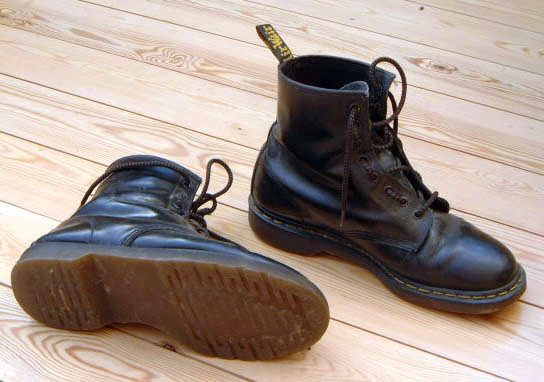
\includegraphics[width=0.8\textwidth,height=\textheight]{Dr_Martens_black_old}

\tiny\{\{\tt http://tradingconsequences.blogs.edina.ac.uk/files/2013/10/Dr\_Martens\_black\_old.jpg\}\}\}
\end{frame}

\begin{frame}
\vspace{2mm}

\begin{itemize}
\tightlist
\item
  Flexible and powerful statistical tool that can be used to quantify
  \emph{uncertainty} associated with an estimator or statistical
  learning method.
\end{itemize}

\vspace{2mm}

\begin{itemize}
\tightlist
\item
  Very popular to obtain standard errors or confidence intervals for a
  coefficient, when parametric theory does not provide it.
\end{itemize}

\vspace{2mm}

\begin{itemize}
\tightlist
\item
  The inventor: Bradley Efron in 1979 -
  \href{https://www.youtube.com/watch?v=6l9V1sINzhE}{see interview}.
\end{itemize}
\end{frame}

\begin{frame}
\begin{itemize}
\tightlist
\item
  The name? \emph{To pull oneself up by one's bootstraps} from ``The
  Surprising Adventures of Baron Munchausen'' by Rudolph Erich Raspe:
\end{itemize}

\(~\)

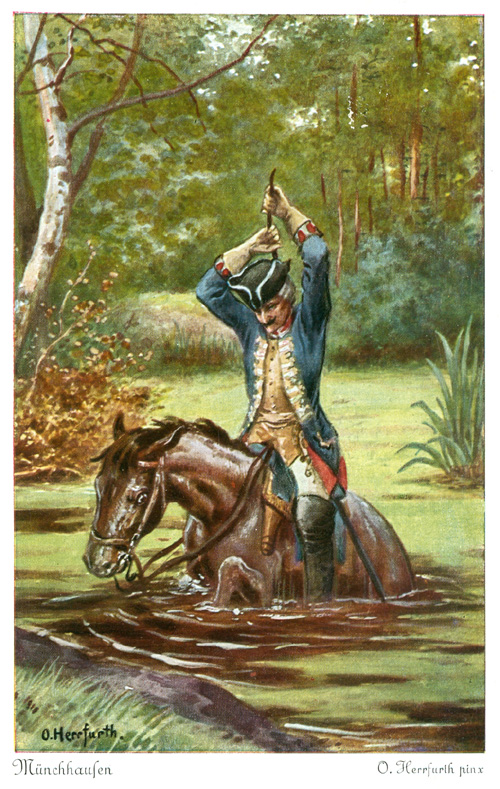
\includegraphics[width=0.2\textwidth,height=\textheight]{muenchhausen}

\begin{quote}
The Baron had fallen to the bottom of a deep lake. Just when it looked
like all was lost, he thought to pick himself up by his own bootstraps.
\end{quote}

\(~\)

\begin{itemize}
\tightlist
\item
  \textbf{Idea: Use the data itself to get more information about a
  statistic (an estimator).}
\end{itemize}
\end{frame}

\begin{frame}{Example}
\protect\hypertarget{example-1}{}
\begin{longtable}[]{@{}llr@{}}
\toprule\noalign{}
Type & Life\_length & Mean \\
\midrule\noalign{}
\endhead
Treatment & 94,197,16,38,99,141,23 & 86.86 \\
Control & 52,104,146,10,51,30,40,27,46 & 56.22 \\
\bottomrule\noalign{}
\end{longtable}

\begin{itemize}
\item
  Is the difference between \emph{means} significant?
\item
  In the difference between \emph{medians} significant?
\end{itemize}
\end{frame}

\begin{frame}
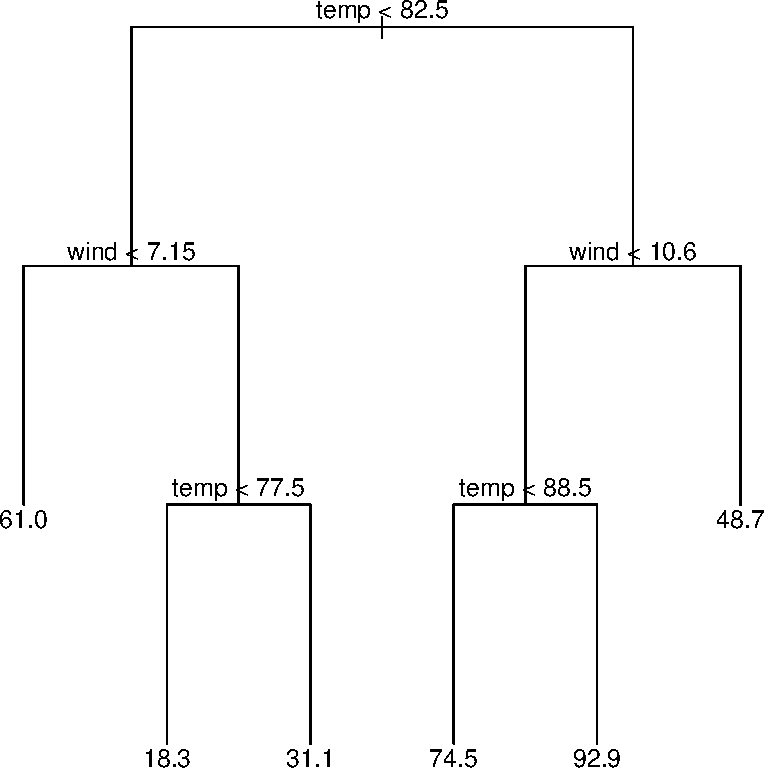
\includegraphics{5Resample_files/figure-beamer/unnamed-chunk-5-1.pdf}
\end{frame}

\begin{frame}
\begin{itemize}
\item
  For the means we can derive analytical solutions but not for the
  median
\item
  If we would know the median distribution \(F\) , we could sample from
  \(F\) , and use simulations to answer our question.
\item
  However, without knowledge of the distribution, we cannot calculate
  the standard deviation of our estimator
\item
  That's where the bootstrap method comes into play
\end{itemize}
\end{frame}

\begin{frame}
\begin{block}{Moving from simulation to bootstrapping (\(f\) unknown)}
\protect\hypertarget{moving-from-simulation-to-bootstrapping-f-unknown}{}
\(~\)

\begin{itemize}
\tightlist
\item
  The bootstrap method is using the observed data to estimate the
  \emph{empirical distribution} \(\hat{f}\), that is each observed value
  of \(x\) is given probability \(1/n\).
\end{itemize}

\vspace{2mm}

\begin{itemize}
\tightlist
\item
  A \emph{bootstrap sample} \(X^*_1,X^*_2,\ldots, X^*_n\) is a random
  sample drawn from \(\hat{f}\).
\end{itemize}

\vspace{2mm}

\begin{itemize}
\tightlist
\item
  A simple way to obtain the bootstrap sample is to \emph{draw with
  replacement from \(X_1, X_2, \ldots, X_n\)}.
\end{itemize}

\vspace{2mm}

\begin{itemize}
\tightlist
\item
  \textbf{Note}: Our bootstrap sample consists of \(n\) members of
  \(X_1, X_2, \ldots, X_n\) - some appearing more than once, other not
  appearing at all.
\end{itemize}
\end{block}
\end{frame}

\begin{frame}[fragile]
Compute one bootstrap sample for the control group \(~\)

The original median: \scriptsize

\begin{Shaded}
\begin{Highlighting}[]
\FunctionTok{set.seed}\NormalTok{(}\DecValTok{123}\NormalTok{)}
\NormalTok{n }\OtherTok{=} \DecValTok{101}
\FunctionTok{print}\NormalTok{(control)}
\end{Highlighting}
\end{Shaded}

\begin{verbatim}
## [1]  52 104 146  10  51  30  40  27  46
\end{verbatim}

\begin{Shaded}
\begin{Highlighting}[]
\FunctionTok{median}\NormalTok{(control)}
\end{Highlighting}
\end{Shaded}

\begin{verbatim}
## [1] 46
\end{verbatim}

\normalsize

The median from \textbf{one bootstrap-sample}: \scriptsize

\begin{Shaded}
\begin{Highlighting}[]
\NormalTok{boot1 }\OtherTok{=} \FunctionTok{sample}\NormalTok{(}\AttributeTok{x =}\NormalTok{ control, }\AttributeTok{size =} \FunctionTok{length}\NormalTok{(control), }\AttributeTok{replace =} \ConstantTok{TRUE}\NormalTok{)}
\FunctionTok{median}\NormalTok{(boot1)}
\end{Highlighting}
\end{Shaded}

\begin{verbatim}
## [1] 51
\end{verbatim}

\normalsize

However, drawing only \emph{one} such sample does not help much.
\end{frame}

\begin{frame}
\begin{block}{The bootstrap algorithm for estimating standard errors}
\protect\hypertarget{the-bootstrap-algorithm-for-estimating-standard-errors}{}
\(~\)

\begin{enumerate}
\tightlist
\item
  Drawing \(B\) bootstrap samples: drawn with replacement from the
  original data.
\end{enumerate}

\vspace{2mm}

\begin{enumerate}
\setcounter{enumi}{1}
\tightlist
\item
  Evaluate the statistic of interest on \emph{each of the \(B\)
  bootstrap samples} to get \(\tilde{X}^*_b\) for the \(b\)th bootstrap
  sample.
\end{enumerate}

\vspace{2mm}

\begin{enumerate}
\setcounter{enumi}{2}
\tightlist
\item
  Estimate squared standard error by
  \[\sqrt{\frac{1}{B-1}\sum_{b=1}^B (\tilde{X}^*_b-\frac{1}{B}\sum_{b=1}^B \tilde{X}^*_b)^2} \ ,\]
  which is the empirical standard deviation from the \(B\) estimates
  \(\tilde{X}^*_b\), \(b=1,\ldots,B\).
\end{enumerate}
\end{block}
\end{frame}

\begin{frame}[fragile]
\begin{block}{Illustration for the median example (with a for-loop in
R)}
\protect\hypertarget{illustration-for-the-median-example-with-a-for-loop-in-r}{}
\(~\)

Simulate data:

\vspace{2mm}

\scriptsize

\begin{Shaded}
\begin{Highlighting}[]
\FunctionTok{set.seed}\NormalTok{(}\DecValTok{123}\NormalTok{)}

\FunctionTok{c}\NormalTok{(}\FunctionTok{median}\NormalTok{(treat), }\FunctionTok{median}\NormalTok{(control))}
\end{Highlighting}
\end{Shaded}

\begin{verbatim}
## [1] 94 46
\end{verbatim}

\(~\)

\normalsize

Then take 1000 bootstrap samples and repeatedly estimate the median to
get a standard deviation:

\vspace{2mm}

\scriptsize

\begin{Shaded}
\begin{Highlighting}[]
\NormalTok{B }\OtherTok{=} \DecValTok{1000}
\NormalTok{estimator\_control }\OtherTok{=}\NormalTok{ estimator\_treat }\OtherTok{=} \FunctionTok{rep}\NormalTok{(}\ConstantTok{NA}\NormalTok{, B)}
\ControlFlowTok{for}\NormalTok{ (b }\ControlFlowTok{in} \DecValTok{1}\SpecialCharTok{:}\NormalTok{B) \{}
\NormalTok{    thisboot }\OtherTok{=} \FunctionTok{sample}\NormalTok{(}\AttributeTok{x =}\NormalTok{ control, }\AttributeTok{size =} \FunctionTok{length}\NormalTok{(control), }\AttributeTok{replace =} \ConstantTok{TRUE}\NormalTok{)}
\NormalTok{    estimator\_control[b] }\OtherTok{=} \FunctionTok{median}\NormalTok{(thisboot)}
\NormalTok{    thisboot }\OtherTok{=} \FunctionTok{sample}\NormalTok{(}\AttributeTok{x =}\NormalTok{ treat, }\AttributeTok{size =} \FunctionTok{length}\NormalTok{(treat), }\AttributeTok{replace =} \ConstantTok{TRUE}\NormalTok{)}
\NormalTok{    estimator\_treat[b] }\OtherTok{=} \FunctionTok{median}\NormalTok{(thisboot)}
\NormalTok{\}}
\FunctionTok{c}\NormalTok{(}\FunctionTok{sd}\NormalTok{(estimator\_control), }\FunctionTok{sd}\NormalTok{(estimator\_treat))}
\end{Highlighting}
\end{Shaded}

\begin{verbatim}
## [1] 13.76477 37.75681
\end{verbatim}
\end{block}
\end{frame}

\begin{frame}
The distribution of the 1000 sampled estimates:

\(~\)

\begin{center}\includegraphics[width=0.7\linewidth]{5Resample_files/figure-beamer/boot2-1} \end{center}
\end{frame}

\begin{frame}[fragile]
\begin{block}{Alternative: the built-in \texttt{boot} function from
library \texttt{boot}}
\protect\hypertarget{alternative-the-built-in-boot-function-from-library-boot}{}
\(~\)

\scriptsize

\begin{Shaded}
\begin{Highlighting}[]
\FunctionTok{library}\NormalTok{(boot)}
\NormalTok{boot.median }\OtherTok{=} \ControlFlowTok{function}\NormalTok{(data, index) }\FunctionTok{return}\NormalTok{(}\FunctionTok{median}\NormalTok{(data[index]))}
\NormalTok{B }\OtherTok{=} \DecValTok{1000}
\FunctionTok{boot}\NormalTok{(control, boot.median, }\AttributeTok{R =}\NormalTok{ B)}
\end{Highlighting}
\end{Shaded}

\begin{verbatim}
## 
## ORDINARY NONPARAMETRIC BOOTSTRAP
## 
## 
## Call:
## boot(data = control, statistic = boot.median, R = B)
## 
## 
## Bootstrap Statistics :
##     original  bias    std. error
## t1*       46  -0.043    12.94592
\end{verbatim}
\end{block}
\end{frame}

\begin{frame}
\begin{block}{With or without replacement?}
\protect\hypertarget{with-or-without-replacement}{}
\vspace{2mm}

In bootstrapping we sample \emph{with replacement} from our
observations.

\vspace{4mm}

\textbf{Q:} What if we instead sample \emph{without replacement}?

\vspace{2mm}

\vspace{4mm}
\end{block}
\end{frame}

\begin{frame}
\begin{block}{Example: multiple linear regression}
\protect\hypertarget{example-multiple-linear-regression}{}
We assume, for observation \(i\):
\[Y_i= \beta_0 + \beta_{1}  x_{i1} + \beta_2 x_{i2} + ... + \beta_p x_{ip} + \varepsilon_i,\]
where \(i=1,2,...,n\). The model can be written in matrix form:
\[{\bf Y}={\bf X} \boldsymbol{\beta}+{\boldsymbol{\varepsilon}}.\]

The least squares estimator:
\(\hat{\boldsymbol\beta}=({\bf X}^T{\bf X})^{-1} {\bf X}^T {\bf Y}\) has
\(\text{Cov}(\boldsymbol\beta)=\sigma^2({\bf X}^T{\bf X})^{-1}\).

In the recommended exercises we will look at how to use bootstrapping to
estimate the covariance of the estimator.\footnote{
Why is that "needed" if we already know the mathematical formula for the standard deviation? Answer: not needed - but OK to look at an example where we know the "truth".}

\vspace{2mm}
\normalsize

\textbf{Note}: Our bootstrap samples can also be used to make confidence
intervals for the regression coefficients or prediction intervals for
new observations.
\end{block}
\end{frame}

\begin{frame}
\begin{itemize}
\tightlist
\item
  Look at the lab in the course book Section 5.3.4.
\end{itemize}

\vspace{2mm}

\begin{itemize}
\tightlist
\item
  In particular: ``Estimating the Accuracy of a Linear Regression
  Model''.
\end{itemize}

\vspace{2mm}

\begin{itemize}
\tightlist
\item
  Why do bootstrap standard errors and theoretical standard errors not
  always correspond? What does that mean?
\end{itemize}
\end{frame}

\begin{frame}
\begin{block}{A related method: Bagging}
\protect\hypertarget{a-related-method-bagging}{}
\vspace{2mm}

Bagging (\emph{bootstrap aggregation}) is a special case of
\emph{ensemble methods}.

\vspace{2mm}

\begin{itemize}
\tightlist
\item
  In Module 8 we will look at bagging, which is built on bootstrapping
  and the fact that it is possible to reduce the variance of a
  prediction by taking the average of many model fits.
\end{itemize}

\vspace{2mm}

\begin{itemize}
\tightlist
\item
  Particularly useful for estimation methods with large variances (like
  regression trees).
\end{itemize}

\vspace{2mm}

\begin{itemize}
\tightlist
\item
  Idea:

  \begin{itemize}
  \tightlist
  \item
    Draw \(B\) bootstrap samples from your data and train the method for
    each sample \(b\) in order to get \(\hat{f}^{\star b}(x)\).
  \item
    Average over all predictions to obtain
    \[\hat{f}_{bag}(x) = \frac{1}{B} \sum_{b=1}^B \hat{f}^{\star b}(x) \ .\]
  \end{itemize}
\end{itemize}
\end{block}
\end{frame}

\begin{frame}
\begin{itemize}
\tightlist
\item
  Like this, we obtain a new model that has a smaller variance than each
  of the individual model. If the bootstrap samples were independent
  (which they are of course not), the variance (thus prediction error)
  would be reduced by
\end{itemize}

\[\text{Var}(\bar{X})=\frac{\sigma^2}{B} \ .\] \vspace{2mm}

\begin{itemize}
\tightlist
\item
  In reality, the variance reduction is less. For a pairwise correlation
  \(\rho\) we would have \(\rho\sigma^2 + \frac{1-\rho}{B}\sigma^2\).
\end{itemize}

\vspace{2mm}

\begin{itemize}
\tightlist
\item
  Models that have poor prediction ability (as we may see can happen
  with regression and classification trees) might benefit greatly from
  bagging. More in Module 8.
\end{itemize}
\end{frame}

\begin{frame}{Further reading}
\protect\hypertarget{further-reading}{}
\begin{itemize}
\tightlist
\item
  \href{https://www.youtube.com/playlist?list=PL5-da3qGB5IA6E6ZNXu7dp89_uv8yocmf}{Videoes
  on YouTube by the authors of ISL, Chapter 5}, and corresponding
  \href{https://lagunita.stanford.edu/c4x/HumanitiesScience/StatLearning/asset/cv_boot.pdf}{slides}
\item
  \href{https://rstudio-pubs-static.s3.amazonaws.com/65561_43c0eaaa8565414eae333b47038f716c.html}{Solutions
  to exercises in the book, chapter 5}
\end{itemize}
\end{frame}

\begin{frame}{Excursion: R Markdown and \texttt{knitr}}
\protect\hypertarget{excursion-r-markdown-and-knitr}{}
\begin{itemize}
\item
  You can work through the Bonus part about R Markdown in the R course
  \url{https://digit.ntnu.no/courses/course-v1:NTNU+IE-IMF+2023_AUG/about}.
\item
  You find a template for the exercise sheets on our course website
  \url{https://wiki.math.ntnu.no/tma4268/2024v/subpage6}. Do not forget
  to install the packages listed at the beginning of the exercise sheet.
\end{itemize}
\end{frame}

\begin{frame}[fragile]
\begin{block}{How to render a document?}
\protect\hypertarget{how-to-render-a-document}{}
\vspace{2mm}

You do this by pressing \texttt{knit}.

Knitting is also done by: Ctrl+Shift+K (Windows) or Cmd+Shift+K (MacOS).

\vspace{2mm}

\begin{enumerate}
[1)]
\item
  Creating documents with R Markdown starts with an .Rmd file that
  contains a combination of markdown (content with simple text
  formatting) and R code chunks.
\item
  The .Rmd file is fed to \texttt{knitr} which executes all of the R
  code chunks and creates a new markdown (.md) document which includes
  the R code and it's output.
\item
  The markdown file generated by \texttt{knitr} is then processed by
  \texttt{pandoc} which is responsible for creating a finished web page,
  PDF, MS Word document, slide show, handout, book, dashboard, package
  vignette or other format.
\end{enumerate}
\end{block}
\end{frame}

\begin{frame}
\begin{itemize}
\item
  More: \href{https://pandoc.org/}{About pandoc - the swiss army knife
  for file conversion}
\item
  NB: even if you write tex this is first translated to md and then via
  pandoc to pdf, so subtle tex stuff may be missed on the way.
\item
  Do you get a separate window popping up, or is your output shown in
  the Viewer tab of one of the window panes? Go to RStudio-Tools-Global
  Options-RMarkdown and check what is your value of ``show output
  preview in''.
\end{itemize}
\end{frame}

\begin{frame}[fragile]
\begin{block}{What output type do you want to produce?}
\protect\hypertarget{what-output-type-do-you-want-to-produce}{}
\vspace{2mm}

\begin{itemize}
\item
  Just keep track of your own work: html\_document
\item
  For TMA4268 Compulsory exercise 1: we ask for a pdf-file (because that
  is easy to read and grade when you upload that to Blackboard)
\item
  To produce a \texttt{pdf\_document} RStudio (using pandoc) will call a
  latex-installation, so you need to have latex installed on your laptop
  to be able to produce a pdf-file.
\item
  Toggle comment/uncomment with hashtag in YAML header \texttt{output}
  to make different options active, then press \texttt{knit}.
  Alterntively this can be done by calling the function
  \texttt{rmarkdown::render()} from your Console window.
\item
  Optional: check that uncommenting \texttt{pdf\_document} and
  commenting out \texttt{html\_document} and pressing \texttt{knit} will
  give you a pdf-file.
\item
  During rendering we use the location of the .Rmd file as the working
  directory, and the rendering is done in a \emph{new session}.
\end{itemize}
\end{block}
\end{frame}

\begin{frame}[fragile]{Formatting your R Markdown file}
\protect\hypertarget{formatting-your-r-markdown-file}{}
\begin{block}{Text, mathematics}
\protect\hypertarget{text-mathematics}{}
\begin{itemize}
\tightlist
\item
  formatted with markdown
\item
  mathematics (in latex) with formulas starting and ending with one
  \texttt{\$} and equation with \texttt{\$\$}
\item
  boldface with two stars and italic with one, new line with two spaces,
\item
  For more, like sections, bulleted or numbered lists, tables,
  footnotes, rulers,\ldots{} see
  \url{https://github.com/rstudio/cheatsheets/raw/master/rmarkdown-2.0.pdf}
\end{itemize}
\end{block}
\end{frame}

\begin{frame}[fragile]
\textbf{Hands-on}: go the the Compulsory exercise 1 template, and just
write and press \texttt{knitr} to see!

Check how a nice formula using latex is generated for
\(Y_i=\beta_0+\beta_1 x_{i1} +\varepsilon_i\).
\end{frame}

\begin{frame}[fragile]
\begin{block}{Code Chunks}
\protect\hypertarget{code-chunks}{}
\(~\)

\begin{itemize}
\tightlist
\item
  Chunks of embedded code. Each chunk begins with ```\{r\} and ends with
  ```
\end{itemize}

\vspace{2mm}

\begin{itemize}
\tightlist
\item
  Set of code chunk options - but I have mainly used these two:

  \begin{itemize}
  \tightlist
  \item
    \texttt{echo}: display the code in the chunk, TRUE or FALSE or
    selected lines, or maybe with an R-object (later)
  \item
    \texttt{eval}: run code in the chunk, TRUE or FALSE
  \end{itemize}
\end{itemize}

\vspace{2mm}

\begin{itemize}
\tightlist
\item
  Remember to include packages to be used within the chunk (only needed
  the first time in a document, if the chung is evaluated,
  \texttt{eval=TRUE}).
\end{itemize}

\vspace{2mm}

\begin{itemize}
\tightlist
\item
  Chunks can have (unique) names, may help when debugging.
\end{itemize}

\vspace{2mm}

\begin{itemize}
\tightlist
\item
  In chunks where figures are generated you can adjust the figure
  width/height and alignment, for example as
\end{itemize}

\texttt{\{r\ auto,\ echo=FALSE,\ fig.width=4,\ fig.height=3,fig.align\ =\ "center",out.width=\textquotesingle{}70\%\textquotesingle{}\}}
\end{block}
\end{frame}

\begin{frame}[fragile]
\begin{block}{Set-up chunk}
\protect\hypertarget{set-up-chunk}{}
\(~\)

\begin{itemize}
\tightlist
\item
  The set-up chunk is a code chunk that you add before you actually
  start to do the work.
\end{itemize}

\vspace{2mm}

\begin{itemize}
\tightlist
\item
  Smart things to add to the setup-chunk:
\end{itemize}

\(~\)

\scriptsize

\begin{Shaded}
\begin{Highlighting}[]
\FunctionTok{library}\NormalTok{(knitr)}
\NormalTok{knitr}\SpecialCharTok{::}\NormalTok{opts\_chunk}\SpecialCharTok{$}\FunctionTok{set}\NormalTok{(}\AttributeTok{echo =} \ConstantTok{TRUE}\NormalTok{, }\AttributeTok{tidy =} \ConstantTok{TRUE}\NormalTok{, }\AttributeTok{message =} \ConstantTok{FALSE}\NormalTok{, }\AttributeTok{warning =} \ConstantTok{FALSE}\NormalTok{,}
    \AttributeTok{strip.white =} \ConstantTok{TRUE}\NormalTok{, }\AttributeTok{prompt =} \ConstantTok{FALSE}\NormalTok{, }\AttributeTok{cache =} \ConstantTok{TRUE}\NormalTok{, }\AttributeTok{size =} \StringTok{"scriptsize"}\NormalTok{,}
    \AttributeTok{fig.width =} \DecValTok{4}\NormalTok{, }\AttributeTok{fig.height =} \DecValTok{3}\NormalTok{)}
\end{Highlighting}
\end{Shaded}
\end{block}
\end{frame}

\begin{frame}[fragile]
\begin{block}{Calling R outside of the code chunks}
\protect\hypertarget{calling-r-outside-of-the-code-chunks}{}
\(~\)

Use the ` r before and ` after an R command to integrate into the text.
For example,

\begin{Shaded}
\begin{Highlighting}[]
\DecValTok{2} \SpecialCharTok{+} \DecValTok{2}
\end{Highlighting}
\end{Shaded}

\begin{verbatim}
## [1] 4
\end{verbatim}

is equal to 4.

\(~\)

This is what we have done in the YAML-header to include todays date on
your submission:

` r format(Sys.time(), `\%d \%B, \%Y')` gives 08 February, 2024.
\end{block}
\end{frame}

\begin{frame}[fragile]{Problems}
\protect\hypertarget{problems}{}
\begin{block}{When I \texttt{knit} with output: pdf\_document no
pdf-file is produced. Why?}
\protect\hypertarget{when-i-knit-with-output-pdf_document-no-pdf-file-is-produced.-why}{}
\begin{itemize}
\tightlist
\item
  html\_document is more forgiving than pdf\_document wrt tex-errors
\item
  a tex-error is not easy to spot - log is terrible
\item
  many students have problems here, and some just end up handing in html
  or Rmd for the projects
\end{itemize}

My solution

\begin{itemize}
\tightlist
\item
  first I render html\_document and look for tex-errors and fix them
\item
  then I render pdf\_document, and include \texttt{keep\_tex:\ yes} yaml
  option
\item
  then I compile the tex in my favorite \texttt{texshop} and look for
  sensible log for errors,
\item
  and then go back to the Rmd and fix the error.
\end{itemize}
\end{block}
\end{frame}

\begin{frame}{Handing in Compulsory exercise 1}
\protect\hypertarget{handing-in-compulsory-exercise-1}{}
\begin{itemize}
\item
  I hope you have already joined a group from Bb (front page -- users
  and groups -- groups).
\item
  Then under Compulsory exercises you will see ``Hand in'' is possible
  (this will come).
\item
  Upload \textbf{both your Rmd and pdf-version of you R Markdown file}
  with your solutions to the exercise (based on the template).
\item
  Scores and comments will be given on Bb.
\end{itemize}
\end{frame}

\begin{frame}
\hypertarget{refs}{}
\begin{CSLReferences}{1}{0}
\leavevmode\vadjust pre{\hypertarget{ref-james.etal}{}}%
James, G., D. Witten, T. Hastie, and R. Tibshirani. 2013. \emph{An
Introduction to Statistical Learning with Applications in r}. New York:
Springer.

\end{CSLReferences}
\end{frame}

\end{document}
